%%%%%%%%%%%%%%%%%%%%%%%%%%%%%
% Standard header for working papers
%
% WPHeader.tex
%
%%%%%%%%%%%%%%%%%%%%%%%%%%%%%

\documentclass[11pt]{article}



%%%%%%%%%%%%%%%%%%%%%%%%%%
%% TEMPLATES
%%%%%%%%%%%%%%%%%%%%%%%%%%


% Simple Tabular

%\begin{tabular}{ |c|c|c| } 
% \hline
% cell1 & cell2 & cell3 \\ 
% cell4 & cell5 & cell6 \\ 
% cell7 & cell8 & cell9 \\ 
% \hline
%\end{tabular}





%%%%%%%%%%%%%%%%%%%%%%%%%%
%% Packages
%%%%%%%%%%%%%%%%%%%%%%%%%%



% encoding 
\usepackage[utf8]{inputenc}
\usepackage[T1]{fontenc}


% general packages without options
\usepackage{amsmath,amssymb,amsthm,bbm}

% graphics
\usepackage{graphicx,transparent,eso-pic}

% text formatting
\usepackage[document]{ragged2e}
\usepackage{pagecolor,color}
%\usepackage{ulem}
\usepackage{soul}


% conditions
\usepackage{ifthen}





%%%%%%%%%%%%%%%%%%%%%%%%%%
%% Maths environment
%%%%%%%%%%%%%%%%%%%%%%%%%%

%\newtheorem{theorem}{Theorem}[section]
%\newtheorem{lemma}[theorem]{Lemma}
%\newtheorem{proposition}[theorem]{Proposition}
%\newtheorem{corollary}[theorem]{Corollary}

%\newenvironment{proof}[1][Proof]{\begin{trivlist}
%\item[\hskip \labelsep {\bfseries #1}]}{\end{trivlist}}
%\newenvironment{definition}[1][Definition]{\begin{trivlist}
%\item[\hskip \labelsep {\bfseries #1}]}{\end{trivlist}}
%\newenvironment{example}[1][Example]{\begin{trivlist}
%\item[\hskip \labelsep {\bfseries #1}]}{\end{trivlist}}
%\newenvironment{remark}[1][Remark]{\begin{trivlist}
%\item[\hskip \labelsep {\bfseries #1}]}{\end{trivlist}}

%\newcommand{\qed}{\nobreak \ifvmode \relax \else
%      \ifdim\lastskip<1.5em \hskip-\lastskip
%      \hskip1.5em plus0em minus0.5em \fi \nobreak
%      \vrule height0.75em width0.5em depth0.25em\fi}



%% Commands

\newcommand{\noun}[1]{\textsc{#1}}


%% Math

% Operators
\DeclareMathOperator{\Cov}{Cov}
\DeclareMathOperator{\Var}{Var}
\DeclareMathOperator{\E}{\mathbb{E}}
\DeclareMathOperator{\Proba}{\mathbb{P}}

\newcommand{\Covb}[2]{\ensuremath{\Cov\!\left[#1,#2\right]}}
\newcommand{\Eb}[1]{\ensuremath{\E\!\left[#1\right]}}
\newcommand{\Pb}[1]{\ensuremath{\Proba\!\left[#1\right]}}
\newcommand{\Varb}[1]{\ensuremath{\Var\!\left[#1\right]}}

% norm
\newcommand{\norm}[1]{\left\lVert #1 \right\rVert}



% argmin
\DeclareMathOperator*{\argmin}{\arg\!\min}


% amsthm environments
\newtheorem{definition}{Definition}
\newtheorem{proposition}{Proposition}
\newtheorem{assumption}{Assumption}

%% graphics

% renew graphics command for relative path providment only ?
%\renewcommand{\includegraphics[]{}}


\usepackage{hyperref}





% geometry
\usepackage[margin=2cm]{geometry}

% layout : use fancyhdr package
\usepackage{fancyhdr}
\pagestyle{fancy}

\makeatletter

\renewcommand{\headrulewidth}{0.4pt}
\renewcommand{\footrulewidth}{0.4pt}
\fancyhead[RO,RE]{\textit{Working Paper}}
\fancyhead[LO,LE]{ISC-PIF}
\fancyfoot[RO,RE] {\thepage}
\fancyfoot[LO,LE] {\noun{J. Raimbault}}
\fancyfoot[CO,CE] {}

\makeatother


%%%%%%%%%%%%%%%%%%%%%
%% Begin doc
%%%%%%%%%%%%%%%%%%%%%

\begin{document}







\title{Exploration methods for Luti models}
\author{}
\date{}


\maketitle

\justify


%\begin{abstract}

%\end{abstract}


%%%%%%%%%%%%%%%%%%%%
\section{Introduction}

\begin{itemize}
	\item Luti model are a very diffuse class of models, dealing mainly with interactions between a land-use system and a transport system, at mesoscopic spatial scales (metropolitan areas) and medium time scales (decades) \cite{raimbault2018phdthesis}. They are developed and used by various scientific fields, from urban economics, network economics to planning and transportation \cite{raimbault:halshs-01584894}.
	\item Despite this sparsity, properties such as the spatial structure of population or the transportation network, or output indicators, can be put in correspondence between most Luti models.
	\item We aim here to illustrate generic methods that could be applied to the exploration of Luti models. 
\end{itemize}


%%%%%%%%%%%%%%%%%%%%
\section{Model}

We use a toy model to illustrate the application of exploration methods. The model Lutecia \cite{lenechet:halshs-01272236} is an extended LUTI with an evolving network following endogenous rules for transportation governance. Blocking the network evolution yields a simplified LUTI (Lowry-type).

\subsection{Model description}

We describe the main features of the simplified LUTI. The metropolitan region is divided into cells, which are characterized by their number of actives $A_i$ and number of employments $E_i$. The total number of actives and employments are fixed during the time period (no growth). At each time step, a proportion $\alpha$ of both relocate following a discrete choice model with parameter $\beta$, following a utility expressed as $X_i^{\gamma_A} \cdot \left(\frac{1}{A_i E_i}\right)^{1 - \gamma_A}$ for actives and $X_i^{\gamma_E}$ for employments, where $\gamma_A,\gamma_E$ are Cobb-Douglas parameters and $X_i$ is the generalized accessibility, computed with an exponential decay of parameter $\lambda$ and with the network distance within a network of uniform speed $v_0$. The evolution is stopped at a fixed final time $t_f$. See \cite{raimbault2018phdthesis} for a more thorough description of the full model.

The model is implemented in NetLogo (\href{https://github.com/JusteRaimbault/Governance}{git repository}) and explored with OpenMOLE.



%%%%%%%%%%%%%%%%%%%%
\subsection{Model evaluation}

\subsubsection{Parameters}

The free Luti parameters are :
\begin{itemize}
	\item $\alpha$ relocation rate
	\item $\lambda$ cost of energy
	\item $\beta$ discrete choice parameter
	\item $\gamma_A$ Cobb-Douglas exponent actives
	\item $\gamma_E$ Cobb-Douglas exponent employments
	\item $v_0$ network speed
\end{itemize}


\subsubsection{Indicators}

We use the following output indicators :
\begin{itemize}
	\item Network indicators (fixed by the scenario and the replication), both contradictory objective for which the network generation heuristic finds a compromise :
	\begin{itemize}
		\item network relative cost : length of the network relative to the length of the full euclidian network between all centers
		\item network performance : \cite{banos2012towards}
	\end{itemize}
	\item Sustainability indicators (should be the objective of PSE / OSE / calibrations). Can be contradictory but not clear :
	\begin{itemize}
		\item Evolution of the average accessibility between initial and final state
		\item Average congestion, approximated by the average weighted betweenness centrality (using stationary commuting flows between actives and employments)
	\end{itemize}
	\item Urban form indicators : four dimensions (moran, average distance, entropy, hierarchy) \cite{2017arXiv170806743R} for population and employments
\end{itemize}


\subsubsection{Setup scenarios}

To be relevant with classical application of LUTI models, we generate typical scenarios for the initial configuration of the model. The initial setup for actives and employments is done in a synthetic way to mimic a polycentric metropolitan are, i.e. with exponential mixtures spatial distributions with common centers, and a slightly higher concentration for employments. We play on the number of centers $N_c$.

Furthermore, a network must be generated, which will be interpreted as the application of the Luti to the design of a new infrastructure. We use the following options to generate a network:
\begin{enumerate}
	\item Random tree-like network: each center connects with an other random center which has no links if there are some. This yield a costly and inefficient network.
	\item Full network: all centers are directly connected. Extreme on the Pareto front: most efficient network, but costly.
	\item Slime-mould biological network generator : applying the results of \cite{raimbault2015labex}, a network reinforcement model mimicking an organism self-organizes into Pareto-efficient networks (in the sense of cost/efficiency and cost/robustness). A single parameter $\gamma$ allows to switch between redundant but costly networks to cheaper but less robust networks.
\end{enumerate}

\textit{We do not add bord nodes and consider the transportation network within the metropolitan area only.}

We currently implement 8 scenarios : (3/5 centers) x (tree/full/cheap slime-mould/robust slime-mould).


\subsubsection{Stylized facts}

Question to answer through the study of sustainability indicators :
\begin{itemize}
  \item compromise between congestion and accessibility across scenarios/parameters ? (attraction-repulsion urban narrative)
  \item Parameters/scenarios to maximize accessibility ?
  \item \textit{less interesting regarding luti : classification of output urban forms ?}
\end{itemize}


Luti stylized facts to be targeted by the model : from \cite{wegener2004land}, some qualitative empirical behavior can be studied in the model.

%  - impact of LU on Transport :
%  o (no mode)    - correlation residential density / transportation mode 
%  o : flows by patch ? (pb : unique mode)    - employment density => more public transport
%  o (no design)    - neighborhood design (e.g. traditional vs car-oriented) influences trip length and modal shares
%  o : flows = f(d) ? no mode    - distance to public transport and employment centers => model shares
%  o (no city size)    - larger cities have highest public transport model share and shorter trips
%  - impact of Transport on LU :
%  x : delta pop = f(access)    - more accessible areas are developed faster
%  x : idem pop    - employments locate in highly accessible areas
%  x : access - sprawl - trip length    - good accessibility => suburban dispersal => longer trips
%  - transport :
%  o (no mode)    - travel cost / travel time => modal choice
%  x : effective distance - trip length    - travel time improvement => more and longer trips (Zahavi law)

\begin{itemize}
	\item ``\textit{more accessible areas are developed faster}'': $\rho\left[X_i,\Delta P_i\right] > 0$
	\item ``\textit{employments locate in highly accessible areas}'': $\rho\left[X_i,E_i\right] > 0$
	\item ``\textit{good access $\implies$ suburban dispersal $\implies$ longer trips}'': $\rho\left[X_i,t_i\right] > 0$ at the scale of a run, $\rho\left[\tilde{X},\alpha_A\right] > 0$ on repetitions
	\item ``\textit{travel time improvement $\implies$ more and longer trips}'': $\rho\left[t_i,d_i\right] < 0$ where $d_i = \sum_j \frac{\phi_{ij}}{\sum_{kl} \phi_{kl}} \cdot d_{ij}$ is the average travel distance from patch i.
\end{itemize}




%%%%%%%%%%%%%%%%%%%%
\section{Results}


\subsection{Sensitivity to indicators and convergence}

\subsubsection{Sensitivity experiment}

\textit{First direct sampling to check the relative sensitivity to parameters, to see if we should fix spatial configurations}

Basic experience plan (\href{https://github.com/JusteRaimbault/Governance/commit/8f848a20abca8c51b927e18c1aaf1ad3434af2cb}{commit 8f848a}) :
LHS for parameters (400) x 6 scenarios x Random spatial configurations (100 repetitions)


\paragraph{Results: anova}

We fit indicators using linear models as a function of parameters and scenario number. An Analysis of Variance shows a comparable sensitivity to scenarios, parameters, and repetitions. Network indicators are as expected mostly sensitive to scenarios.

% anova results
%             betaDC            gammaCDA            gammaCDE           lambdaAcc      relocationRate        networkSpeed 
%          0.1055526           0.6849464           0.4647941          45.7127247           2.2179705          23.1167898 
%as.factor(scenario)           Residuals 
%          7.2665224          20.4306995 

\begin{table}
\caption{ANOVA of the direct sampling experiment}
\begin{center}
\begin{tabular}{|c|c|c|c|c|c|c|c|c|}
\hline
Parameter & $\beta$ & $\gamma_A$ & $\gamma_E$ & $\lambda$ & $\alpha$ & $v_0$ & scenario & residuals \\
\% variance & 0.11 & 0.68 & 0.46 & 45.71 & 2.22 & 23.12 & 7.27 & 20.43 \\
\hline
\end{tabular}
\end{center}
\end{table}

Since the most influent parameters for relative accessibility are the cost of energy $\lambda$ and the network speed $v_0$, and since these are relatively exogenous factors (compared to the governable parameters within the region e.g.), we fix them in following experiments to standard values of $\lambda = 0.005$ and $v_0 = 5$.


\paragraph{Results: repetitions}

To have a rough ideas of the number of repetitions needed to reach a given confidence interval on averages, we consider the relative accessibility $\tilde{X}$. Distributions can roughly be approximated as Gaussians (see Fig.~\ref{fig:distrib-access}), and we can use the formula giving the size of the confidence interval around the mean as $2\sigma z_{level} / \sqrt{n}$.

Looking at the distribution of $\frac{c_i + c_j}{\left|m_i - m-j\right|}$ for all $(i,j)$, where $c_i$ and $c_j$ are half-width of confidence intervals and $m_i,m_j$ the average estimated values, we find that the 97.5\% centile corresponds to value of 0.96, what means that a large majority of estimated values can be tell apart at a 95\% confidence level.


%%%%%%%%%%%%%%
\begin{figure}
	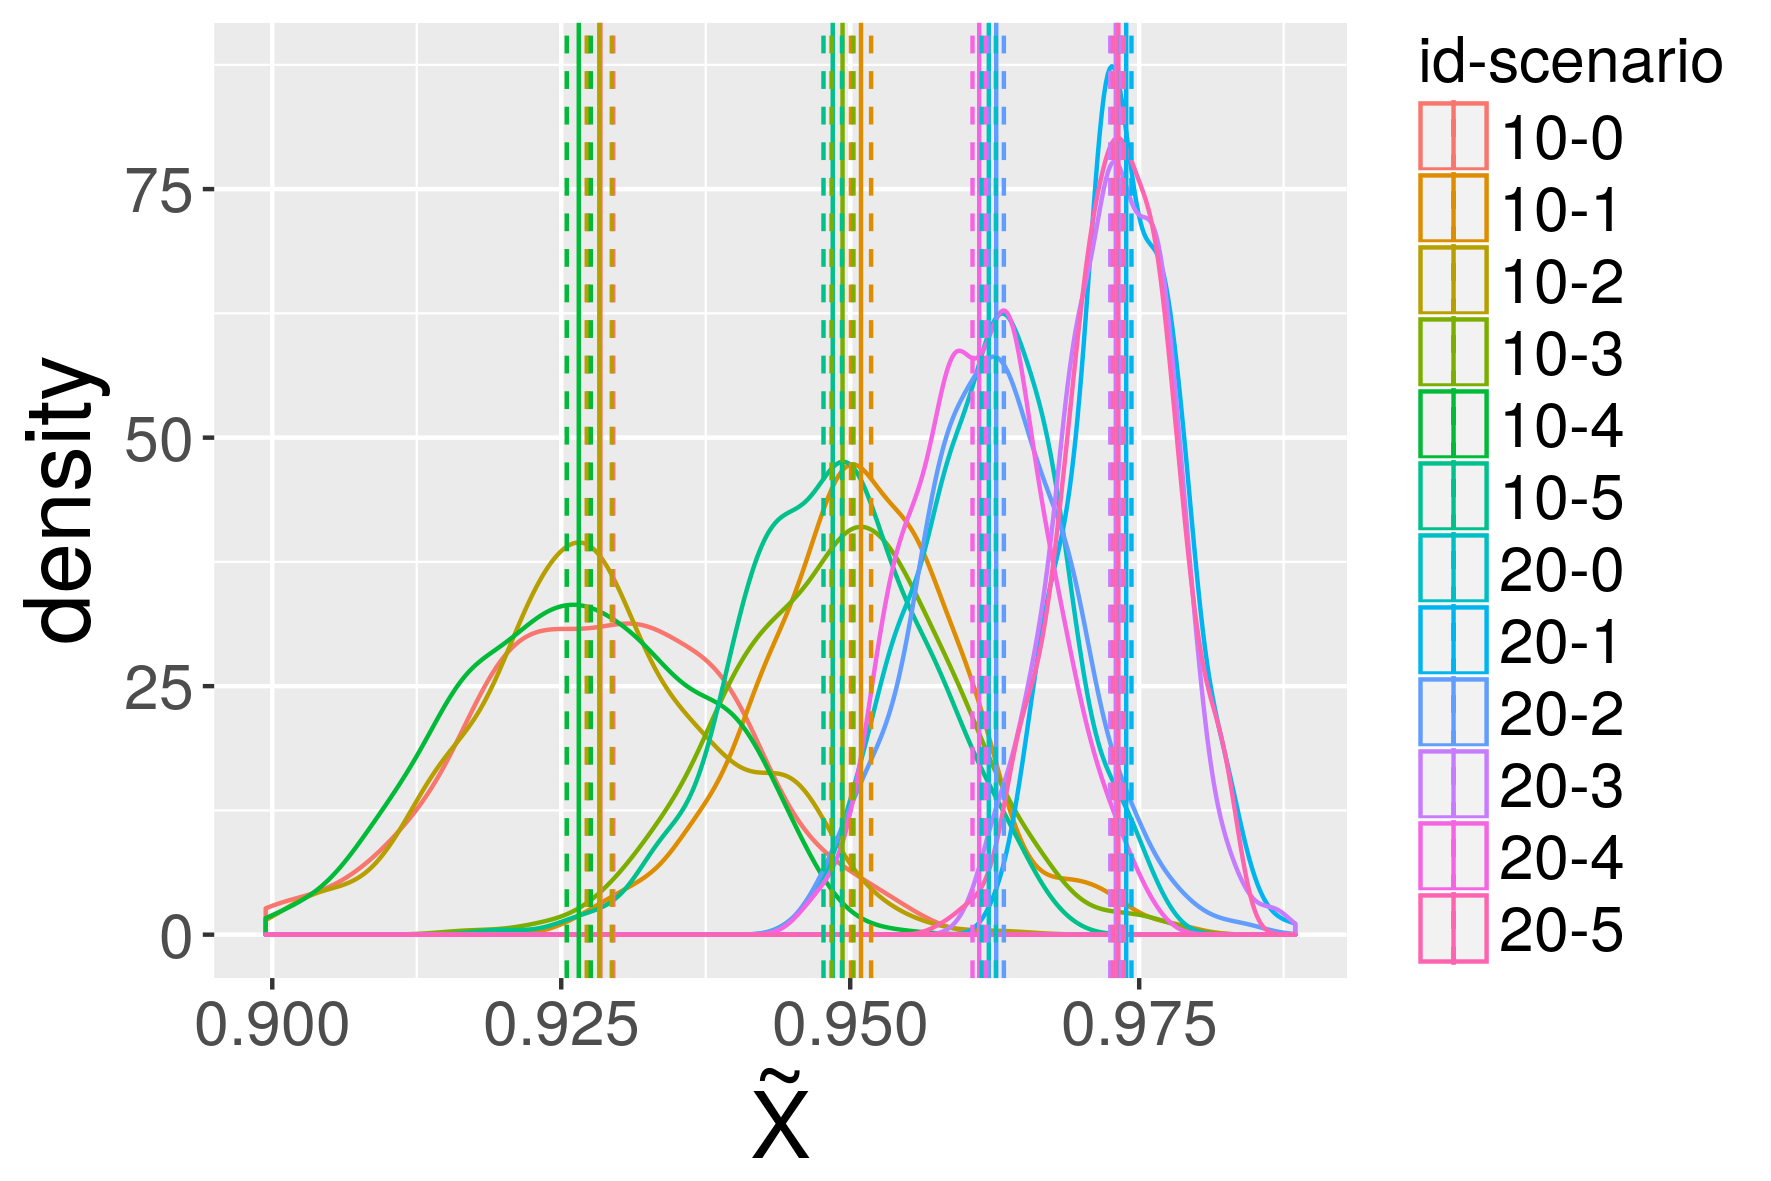
\includegraphics[width=\textwidth]{figures/20180417_184334_SPACEMATTERS_distrib_relativeAccessibility.png}
	\caption{Distribution of relative accessibility $\tilde{X}$ for two example parameter values and the 6 scenarios (parameter point 10 corresponds to $\beta = 1.71,\gamma_A=0.787,\gamma_E=0.798,\lambda=0.00572,v_0=4.15,\alpha=0.96$, parameter point 20 to $\beta = 0.74,\gamma_A=0.92,\gamma_E=0.70,\lambda=0.0045,v_0=2.72,\alpha=0.74$).\label{fig:distrib-access}}
\end{figure}



\subsubsection{Refined experiment}

\textit{Similar experience plan, with fixed $\lambda$ and $v_0$, additional scenarios (complete network), and a weighted congestion indicator.} (\href{https://github.com/JusteRaimbault/Governance/commit/26f7f77b9a4fc378a0985de4493fe94a50846ce4}{commit 26f7f7}) :

200 replications x 500 parameter points (LHS) x 8 scenarios






\paragraph{Behavior in comparison to reference}

\textit{TODO : compare tree and full network scenarios to the slime mould}




%%%%%%%%%%%%%%%%
\subsection{PSE}

\textit{PSE to launch separately on sustainability/urban form - decide if across scenarios or if scenario as discrete genome}


\subsection{OSE}

\textit{experiment Romain}



\subsection{Space matters}

\textit{Experiments testing various urban structure - similar to scenarios in the first sensitivity experiment but broader.}




%%%%%%%%%%%%%%%%%%%%
%% Biblio
%%%%%%%%%%%%%%%%%%%%

\bibliographystyle{apalike}
\bibliography{/home/raimbault/ComplexSystems/CityNetwork/Biblio/Bibtex/CityNetwork.bib,/home/raimbault/ComplexSystems/CityNetwork/Biblio/Bibtex/selfcit.bib,/home/raimbault/ComplexSystems/SimulationModels/Biblio/SimulationModels.bib}


\end{document}
